\section{Ôn tập chương 6 - Mũ - Logarit}
\Opensolutionfile{ans}[ans/ans-OTC6-TN]
\caulc
\begin{ex}%Câu 1.%[1D6H1-2]
	Viết biểu thức $P=\sqrt[3]{x\cdot\sqrt[4]{x}}$, $(x>0)$ dưới dạng lũy thừa với số mũ hữu tỷ. 
	\choice
	{$P=x^{\tfrac{5}{4}}$}
	{$P=x^{\tfrac{1}{12}}$}
	{\True $P=x^{\tfrac{5}{12}}$}
	{$P=x^{\tfrac{1}{7}}$}
	\loigiai{
		Ta có $P=\sqrt[3]{x\cdot\sqrt[4]{x}}=\sqrt[3]{x\cdot x^{\tfrac{1}{4}}}=\sqrt[3]{x^{\tfrac{5}{4}}}=x^{\tfrac{5}{12}}$.}
\end{ex}
\begin{ex}%Câu 2.%[1D6N3-2]
	Tập xác định của hàm số $y=\log_2(x-1)$ là
	\choice
	{$(2;+\infty)$}
	{$(-\infty;+\infty)$}
	{\True $(1;+\infty)$}
	{$(-\infty;1)$}
	\loigiai{
		Điều kiện xác định $x-1>0\Leftrightarrow x>1$.\\
		Vậy tập xác định của hàm số $y=\log_2(x-1)$ là $(1;+\infty)$.}
\end{ex}
\begin{ex}%Câu 3.%[1D6H2-2]
	Cho $\log_25=a$; $\log_53=b$. Tính $\log_524$ theo $a$ và $b$. 
	\choice
	{\True $\log_524=\dfrac{3+ab}{a}$}
	{$\log_524=\dfrac{a+3b}{a}$}
	{$\log_524=\dfrac{3a+b}{b}$}
	{$\log_524=\dfrac{a+b}{3ab}$}
	\loigiai{
		Ta có \allowdisplaybreaks \begin{eqnarray*}
			\log_524&=&\log_5(8\cdot 3)=\log_58+\log_53\\
			&=&3\cdot\log_52+\log_53=\dfrac{3}{\log_25}+\log_53\\
			&=&\dfrac{3}{a}+b=\dfrac{3+ab}{a}.
			\end{eqnarray*}
		}
\end{ex}
\begin{ex}%Câu 4.%[1D6N2-2]
	Với mọi số thực $a$ dương, $\log_4a^4$ bằng
	\choice
	{$4$}
	{$\dfrac{1}{4}$}
	{$\dfrac{1}{4}\log_4a$}
	{\True $4\log_4a$}
	\loigiai{
		Ta có $\log_4a^4=4\log_4|a|=4\log_4a$.}
\end{ex}
\begin{ex}%Câu 5.%[1D6N2-2]
	Giá trị của biểu thức $4^{\log_2\sqrt{3}}$ bằng
	\choice
	{\True $3$}
	{$\sqrt{3}$}
	{$2^{\sqrt{3}}$}
	{$2\sqrt{3}$}
	\loigiai{
		Ta có $4^{\log_2\sqrt{3}}=(2^2)^{\log_2\sqrt{3}}=\left(2^{\log_2\sqrt{3}}\right)^2=(\sqrt{3})^2=3$.}
\end{ex}
\begin{ex}%Câu 6.%[1D6N3-3]
	Trong bốn hàm số sau, hàm số nào nghịch biến trên $\mathbb{R}$?
	\choice
	{$y=2024^x$}
	{$y=\left(\dfrac{2024}{2023}\right)^x$}
	{$y=\log_{2024}x$}
	{\True $y=\left(\dfrac{2023}{2024}\right)^x$}
	\loigiai{
		Hàm số $y=\left(\dfrac{2023}{2024}\right)^x$ nghịch biến trên $\mathbb{R}$ do cơ số $\dfrac{2023}{2024}\in(0; 1)$.}
\end{ex}
\begin{ex}%Câu 7.%[1D6H4-2]
	Nghiệm của phương trình $\log_2(3x-4)=-1$ là
	\choice
	{$x=2$}
	{$x=\dfrac{7}{6}$}
	{\True $x=\dfrac{3}{2}$}
	{$x=\dfrac{5}{3}$}
	\loigiai{
		Ta có $\log_2(3x-4)=-1\Leftrightarrow 3x-4=2^{-1}=\dfrac{1}{2}\Leftrightarrow x=\dfrac{3}{2}$.}
\end{ex}
\begin{ex}%Câu 8.%[1D6H3-3]
	\immini{
		Cho hàm số $y=\log_ax\left(a>0, a\neq 1\right)$ có đồ thị như hình vẽ. Giá trị của $a$ bằng
	\choice
	{$a=2$}
	{$a=\sqrt{2}$}
	{$a=\dfrac{1}{\sqrt{2}}$}
	{\True $a=\dfrac{1}{2}$}
	}{
		\begin{tikzpicture}[scale=0.7, font=\footnotesize, line join=round, line cap=round,>=stealth]
			\def\xmax{5} \def\ymin{-3} \def\ymax{3}
			\draw[->] (-0.9,0)--(\xmax,0) node [below]{$x$};
			\draw[->] (0,\ymin)--(0,\ymax) node [left]{$y$};
			\node at (0,0) [above left]{$O$};
			\clip (-0.9,\ymin) rectangle (\xmax-0.1,\ymax-0.1);
			\draw[smooth,samples=300,domain=0.03:\xmax] plot(\x,{ln(\x)/ln(0.5)});
			\draw[dashed] (2,0)node[above]{$2$}--(2,-1)--(0,-1)node[left]{$-1$};
			\fill (1,0) circle (1.0pt) node[below]{$1$} (2,0) circle (1.0pt) (0,-1) circle (1.0pt);
		\end{tikzpicture}		
	}
	\loigiai{
		Đồ thị hàm số $y=\log_ax$ đi qua điểm $(2;-1)$ nên $\log_a2=-1$.\\
		Khi đó $a^{-1}=2\Leftrightarrow\dfrac{1}{a}=2\Leftrightarrow a=\dfrac{1}{2}$.}
\end{ex}
\begin{ex}%Câu 9.%[1D6H4-4]
	Số nghiệm thực của phương trình $3\log_3(x-1)-\log_{\tfrac{1}{3}}(x-5)^3=3$ là
	\choice
	{$3$}
	{$2$}
	{\True $1$}
	{$0$}
	\loigiai{
		Điều kiện: $x>5$.\\
		Ta có \allowdisplaybreaks\begin{eqnarray*}
			&&3\log_3(x-1)-\log_{\tfrac{1}{3}}(x-5)^3=3\\
			&\Leftrightarrow& 3\log_3(x-1)+3\log_3(x-5)=3 \\
		 &\Leftrightarrow&\log_3(x-1)+\log_3(x-5)=1\\
		 &\Leftrightarrow&\log_3[(x-1)(x-5)]=1\\
		 &\Leftrightarrow&(x-1)(x-5)=3  \\
		& \Leftrightarrow& x^2-6x+2=0\Leftrightarrow x=3\pm\sqrt{7}.
		\end{eqnarray*}
		Đối chiếu điều kiện suy ra phương trình có $1$ nghiệm $x=3+\sqrt{7}$.}
\end{ex}
\begin{ex}%Câu 10.%[1D6V3-2]
	Số các giá trị nguyên dương của tham số $m$ để hàm số\\ $f(x)=\log_{2024}\left[x^2-2(m-1)x-m^2+3m+8\right]$ xác định với mọi giá trị thực của $x$. 
	\choice
	{$4$}
	{$2$}
	{\True $3$}
	{$1$}
	\loigiai{
		Ta thấy hàm số $f(x)=\log_{2024}\left[x^2-2(m-1)x-m^2+3m+8\right]$ xác định với mọi giá trị thực của $x$ khi và chỉ khi $x^2-2(m-1)x-m^2+3m+8>0,\forall x\in\mathbb{R}$ \\
		$ \Leftrightarrow\heva{&1>0\\&\Delta’=(m-1)^2-\left(-m^2+3m+8\right)<0}\Leftrightarrow 2m^2-5m-7<0\Leftrightarrow-1<m<\dfrac{7}{2}$. \\
		Do $m\in\mathbb{N}^*$ nên $m\in\{1;2;3\}$.\\
		Vậy có $3$ giá trị nguyên dương của tham số $m$ thoả mãn yêu cầu bài toán.}
\end{ex}
\begin{ex}%Câu 11.%[1D6V3-3]
	\immini{
		Cho các hàm số $y=\log_ax$; $y=\log_bx$; $y=\log_cx$ có đồ thị như hình vẽ. Khẳng định nào sau đây đúng?
	\choice
	{\True $a>c>b$}
	{$a>b>c$}
	{$c>a>b$}
	{$b>c>a$}
	}{
		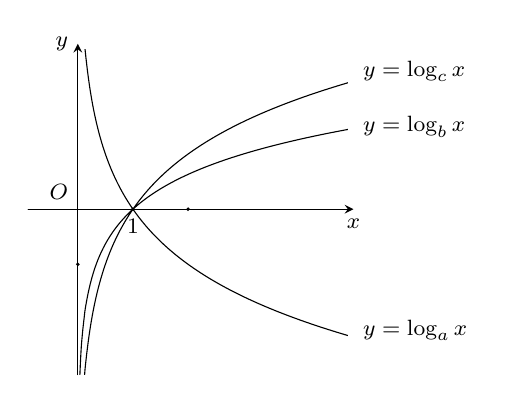
\begin{tikzpicture}[scale=0.7, font=\footnotesize, line join=round, line cap=round,>=stealth]
			\def\xmax{5} \def\ymin{-3} \def\ymax{3}
			\draw[->] (-0.9,0)--(\xmax,0) node [below]{$x$};
			\draw[->] (0,\ymin)--(0,\ymax) node [left]{$y$};
			\node at (0,0) [above left]{$O$};
			\node at (5,-2.2) [right]{$y=\log_ax$};
			\node at (5,1.5) [right]{$y=\log_bx$};
			\node at (5,2.5) [right]{$y=\log_cx$};
			\clip (-0.9,\ymin) rectangle (\xmax-0.1,\ymax-0.1);
			\draw[smooth,samples=300,domain=0.03:\xmax] plot(\x,{ln(\x)/ln(0.5)})
			plot(\x,{ln(\x)/ln(2)}) plot(\x,{ln(\x)/ln(3)});
			\fill (1,0) circle (1.0pt) node[below]{$1$} (2,0) circle (1.0pt) (0,-1) circle (1.0pt);			
		\end{tikzpicture}	
	}
	\loigiai{
		Dựa vào đồ thị ta có hàm số $y=\log_bx$ là một hàm số nghịch biến trên tập xác định của nó nên $0<b<1$; hàm số $y=\log_ax$; $y=\log_cx$ là các hàm số đồng biến trên tập xác định của nó nên $a>1$ và $c>1$. 
		\begin{center}
			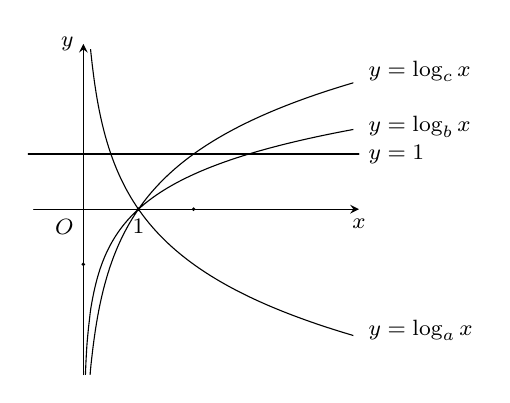
\begin{tikzpicture}[scale=0.7, font=\footnotesize, line join=round, line cap=round,>=stealth]
				\def\xmax{5} \def\ymin{-3} \def\ymax{3}
				\draw[->] (-0.9,0)--(\xmax,0) node [below]{$x$};
				\draw[->] (0,\ymin)--(0,\ymax) node [left]{$y$};
				\node at (0,0) [below left]{$O$};
				\node at (5,-2.2) [right]{$y=\log_ax$};
				\node at (5,1.5) [right]{$y=\log_bx$};
				\node at (5,2.5) [right]{$y=\log_cx$};
				\draw (-1,1)--(5,1)node[right]{$y=1$};	
				\clip (-0.9,\ymin) rectangle (\xmax-0.1,\ymax-0.1);
				\draw[smooth,samples=300,domain=0.03:\xmax] plot(\x,{ln(\x)/ln(0.5)})
				plot(\x,{ln(\x)/ln(2)}) plot(\x,{ln(\x)/ln(3)});
				\fill (1,0) circle (1.0pt) node[below]{$1$} (2,0) circle (1.0pt) (0,-1) circle (1.0pt);				
			\end{tikzpicture}
		\end{center}
		Kẻ đường thẳng $y=1$ cắt đồ thị các hàm số $y=\log_cx$; $y=\log_ax$ lần lượt tại các điểm $A(c; 1)$ và $B(a; 1)$.\\
		Dựa vào đồ thị ta thấy $x_A<x_B\Leftrightarrow c<a$.\\
		Vậy $a>c>b$.}
\end{ex}
\begin{ex}%Câu 12.%[1D6H4-3]
	Bất phương trình $\log_{2024}(x+3)-1\leq 0$ có bao nhiêu nghiệm nguyên dương?
	\choice
	{$2022$}
	{\True $2021$}
	{$2023$}
	{$2024$}
	\loigiai{
		Điều kiện: $x >-3$.\\
		Ta có $\log_{2024}(x+3)-1\leq 0\Leftrightarrow\log_{2024}(x+3)\leq 1\Leftrightarrow x+3\leq 2024\Leftrightarrow x\leq 2021$.\\
		Vì $x\in\mathbb{N}^{*}$ và $x >-3$ nên $x\in\left\{1; 2;\ldots; 2021\right\}$.\\
		Vậy bất phương trình đã cho có $2021$ nghiệm nguyên dương.}
\end{ex}
\Closesolutionfile{ans}
\indapan{6}{ans/ans-OTC6-TN}

\cauds
\Opensolutionfile{ans}[ans/ans-OTC6-DS]
\setcounter{ex}{0}
\begin{ex}%Câu 1.%[1D6V3-3]
	\immini{
		Cho các đồ thị hàm số $y=\log_ax,y=\log_bx,y=\log_cx$ ở hình vẽ. Khẳng định nào sau đây đúng?
	\choiceTF
	{\True $a>1$}
	{\True $0<c<1<a<b$}
	{$\left(a^3\sqrt{a}\right)^{\log_ab}=\sqrt[3]{b^2}$}
	{$P=\log\dfrac{a}{b}+\log\dfrac{b}{c}+\log\dfrac{c}{d}-\log\dfrac{a}{d}>0$ với $d>0$}
	}{
		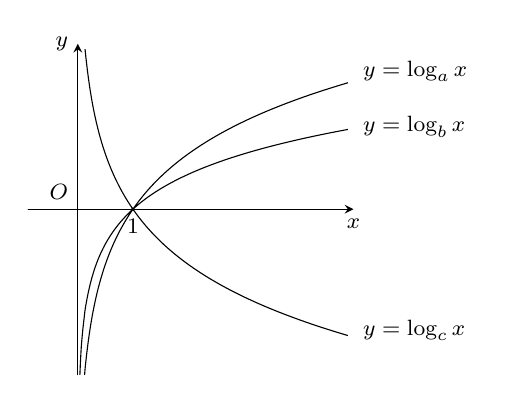
\begin{tikzpicture}[scale=0.7, font=\footnotesize, line join=round, line cap=round,>=stealth]
			\def\xmax{5} \def\ymin{-3} \def\ymax{3}
			\draw[->] (-0.9,0)--(\xmax,0) node [below]{$x$};
			\draw[->] (0,\ymin)--(0,\ymax) node [left]{$y$};
			\node at (0,0) [above left]{$O$};
			\node at (5,-2.2) [right]{$y=\log_cx$};
			\node at (5,1.5) [right]{$y=\log_bx$};
			\node at (5,2.5) [right]{$y=\log_ax$};
			\clip (-0.9,\ymin) rectangle (\xmax-0.1,\ymax-0.1);
			\draw[smooth,samples=300,domain=0.03:\xmax] plot(\x,{ln(\x)/ln(0.5)})
			plot(\x,{ln(\x)/ln(2)}) plot(\x,{ln(\x)/ln(3)});
			\fill (1,0) circle (1.0pt) node[below]{$1$};			
		\end{tikzpicture}
	}
	\loigiai{
		\begin{itemchoice}
		\itemch Đúng. Ta thấy hàm số $y=\log_ax$ đồng biến nên $a>1$.
		\itemch Đúng. Từ đồ thị ta cũng có hàm số $y=\log_bx$ đồng biến nên $b>1$ và hàm số $y=\log_cx$ nghịch biến nên $0<c<1$.\\
		Mặt khác dựng đường thẳng $y=1$ nó cắt hai đồ thị hàm số $y=\log_ax$ và $y=\log_bx$ tại các điểm có hành độ là $a$ và $b$ tương ứng, suy ra $a<b$.\\
		Từ đó ta được $0<c<1<a<b$.
		\itemch Sai. Ta có $\left(a^3\sqrt{a}\right)^{\log_ab}=\left(a^3\cdot a^{\tfrac{1}{2}}\right)^{\log_ab}=\left(a^{\tfrac{7}{2}}\right)^{\log_ab} =\left(a^{\log_ab}\right)^{\tfrac{7}{2}}=b^{\tfrac{7}{2}}=\sqrt{b^7}$. 
		\itemch Sai. Ta có $P=\log\left(\dfrac{a}{b}\cdot\dfrac{b}{c}\cdot\dfrac{c}{d}\right)-\log\dfrac{a}{d}=\log\left(\dfrac{a}{d}\colon\dfrac{a}{d}\right)=\log 1=0$. 
	\end{itemchoice}}
\end{ex}
\begin{ex}%Câu 2.%[1D6N3-2]%[1D6V2-2]
	Cho hàm số $f(x)=\dfrac{1}{2}\log_2\left(\dfrac{2x}{1-x}\right)$.
	\choiceTF
	{\True Tập xác định của hàm số là $\mathscr{D}=(0; 1)$}
	{$f\left(\dfrac{2}{3}\right)=\dfrac{1}{3}$}
	{\True $f(x)+f(1-x)=1$ với mọi $x\in(0; 1)$}
	{\True $f\left(\dfrac{1}{2025}\right)+f\left(\dfrac{2}{2025}\right)+f\left(\dfrac{3}{2025}\right)+\cdots +f\left(\dfrac{2023}{2025}\right)+f\left(\dfrac{2024}{2025}\right)=1012$}
	\loigiai{
		\begin{itemchoice}
		\itemch Đúng. Hàm số xác định $\dfrac{2x}{1-x}>0\Leftrightarrow 2x(1-x)>0\Leftrightarrow 0<x<1$. Vậy tập xác định của hàm số là $\mathscr{D}=(0; 1)$.
		\itemch  Sai. Ta có $f\left(\dfrac{2}{3}\right)=\dfrac{1}{2}\log_2\left(\dfrac{2\cdot\dfrac{2}{3}}{1-\dfrac{2}{3}}\right)=\dfrac{1}{2}\log_2\left(\dfrac{\dfrac{4}{3}}{\dfrac{1}{3}}\right)=\dfrac{1}{2}\log_24=\dfrac{1}{2}\cdot 2=1$.
		\itemch Đúng. Với mọi $x\in(0; 1)$ ta có \allowdisplaybreaks\begin{eqnarray*}
			f(x)+f(1-x)&=&\dfrac{1}{2}\log_2\left(\dfrac{2x}{1-x}\right)+\dfrac{1}{2}\log_2\left[\dfrac{2(1-x)}{1-(1-x)}\right]\\
		&=&\dfrac{1}{2}\log_2\left(\dfrac{2x}{1-x}\right)+\dfrac{1}{2}\log_2\left[\dfrac{2(1-x)}{x}\right]\\
		&=&\dfrac{1}{2}\log_2\left[\dfrac{2x}{1-x}\cdot\dfrac{2(1-x)}{x}\right]=\dfrac{1}{2}\log_24=1.
		\end{eqnarray*}
		\itemch Đúng. Áp dụng tính chất trên, ta được
		\allowdisplaybreaks\begin{eqnarray*}
			S&=&\left[f\left(\dfrac{1}{2025}\right)+f\left(\dfrac{2024}{2025}\right)\right]+\left[f\left(\dfrac{2}{2025}\right)+f\left(\dfrac{2023}{2025}\right)\right]+\\
			&&\cdots +\left[f\left(\dfrac{1012}{2025}\right)+f\left(\dfrac{1013}{2025}\right)\right]\\
		&=&1+1+\cdots +1=1012.
			\end{eqnarray*}
	\end{itemchoice}}
\end{ex}
\begin{ex}%Câu 3.%[1D6V2-2]
	Cho hàm số $f(x)=\log_a(x+1)$ với $a=2024!$. Các mệnh đề sau đúng hay sai?
	\choiceTF
	{$f(0)=1$}
	{Hàm số xác định trên $\mathscr{D}=(0;+\infty)$}
	{$f(x)<1\Leftrightarrow x<2024!-1$}
	{\True $f(1)+f(2)+\cdots +f(2023)=1$}
	\loigiai{
		\begin{itemchoice}
		\itemch Sai. $f(0)=\log_a1=0$ nên mệnh đề sai.
		\itemch Sai. Hàm số xác định khi và chỉ khi $x+1>0\Leftrightarrow x >-1$.
		\itemch Sai. $f(x)<1\Leftrightarrow\log_a(x+1)<1\Leftrightarrow 0<x+1<a\Leftrightarrow-1<x<2024!-1$.
		\itemch Đúng. \allowdisplaybreaks\begin{eqnarray*}
			&&f(1)+f(2)+\cdots +f(2023)\\
			&=&\log_a2+\log_a3+\cdots +\log_a2024\\
			&=&\log_a(2\cdot 3\cdots 2024)=\log_aa=1.
				\end{eqnarray*}
	\end{itemchoice}}
\end{ex}
\begin{ex}%Câu 4.%[1D6N3-2]%[1D6V2-2]
	Cho hàm số $f(x)=\mathrm{e}^{\tfrac{1}{x^2+x}}$. Các mệnh đề sau đúng hay sai?
	\choiceTF
	{\True $f(1)=\sqrt{\mathrm{e}}$}
	{\True Hàm số xác định trên $\mathscr{D}=\mathbb{R}\setminus\{-1;0\}$}
	{Bất phương trình $f(x)<1$ có $2$ nghiệm nguyên}
	{$f(1)\cdot f(2)\cdots f(2024)=\dfrac{2024}{2025}$}
	\loigiai{
		\begin{itemchoice}
		\itemch Đúng. $f(1)=\mathrm{e}^{\tfrac{1}{2}}=\sqrt{\mathrm{e}}$.
		\itemch Đúng. Hàm số xác định khi và chỉ khi $x^2+x\neq 0\Leftrightarrow\heva{&x\neq 0\\&x\neq-1.}$
		\itemch Sai. $f(x)<1\Leftrightarrow\mathrm{e}^{\tfrac{1}{x^2+x}}<1\Leftrightarrow\dfrac{1}{x^2+x}<0\Leftrightarrow x^2+x<0\Leftrightarrow-1<x<0$.
		\itemch Sai. Ta có $f(x)=\mathrm{e}^{\tfrac{1}{x^2+x}}\Rightarrow\ln f(x)=\dfrac{1}{x^2+x}=\dfrac{1}{x}-\dfrac{1}{x+1}$. \\
Khi đó,	 \allowdisplaybreaks\begin{eqnarray*}
		 \ln f(1)+\ln f(2)+\cdots +\ln f(2024)&=&\left(1-\dfrac{1}{2}\right)+\left(\dfrac{1}{2}-\dfrac{1}{3}\right)+\cdots +\left(\dfrac{1}{2024}-\dfrac{1}{2025}\right)\\
		 &=&1-\dfrac{1}{2025} =\dfrac{2024}{2025}.
			\end{eqnarray*}
		Nên $\ln\left[f(1)\cdot f(2)\cdots f(2024)\right]=\dfrac{2024}{2025}\Leftrightarrow f(1)\cdot f(2)\cdots f(2024)=\mathrm{e}^{\tfrac{2024}{2025}}$.
	\end{itemchoice}}
\end{ex}
\Closesolutionfile{ans}
\indapan{3}{ans/ans-OTC6-DS}

\Opensolutionfile{ans}[ans/ans-OTC6-KQ]
\caukq
\setcounter{ex}{0}
\begin{ex}%Câu 1.%[1D6H1-2]
	Cho hai số thực dương $a$, $b$. Rút gọn biểu thức $A=\dfrac{a^{\tfrac{1}{3}}\sqrt{b}+b^{\tfrac{1}{3}}\sqrt{a}}{\sqrt[6]{a}+\sqrt[6]{b}}$, ta được $A=a^m\cdot b^n$. Tính $S=3m+6n$.
	\shortans{$3$}	
	\loigiai{
		$A=\dfrac{a^{\tfrac{1}{3}}\sqrt{b}+b^{\tfrac{1}{3}}\sqrt{a}}{\sqrt[6]{a}+\sqrt[6]{b}}=\dfrac{a^{\tfrac{1}{3}}\cdot b^{\tfrac{1}{2}}+b^{\tfrac{1}{3}}\cdot a^{\tfrac{1}{2}}}{a^{\tfrac{1}{6}}+b^{\tfrac{1}{6}}}=\dfrac{a^{\tfrac{1}{3}}\cdot b^{\tfrac{1}{3}}\left(b^{\tfrac{1}{6}}+a^{\tfrac{1}{6}}\right)}{a^{\tfrac{1}{6}}+b^{\tfrac{1}{6}}}=a^{\tfrac{1}{3}}\cdot b^{\tfrac{1}{3}}$.\\
		Suy ra $m=\dfrac{1}{3}$, $n=\dfrac{1}{3}\Rightarrow 3m+6n=3$.\\
	}
\end{ex}
\begin{ex}%Câu 2.%[1D6V2-3]
	Cho $a$, $b$, $x>0$; $a>b$ và $b$, $x\neq 1$ thỏa mãn $\log_x\dfrac{a+2b}{3}=\log_x\sqrt{a}+\dfrac{1}{\log_bx^2}$. Khi đó biểu thức $P=\dfrac{2a^2+3ab+b^2}{(a+2b)^2}$ có giá trị bằng
	\shortans{$1{,}25$}
	\loigiai{	Ta có \allowdisplaybreaks\begin{eqnarray*}
		&&\log_x\dfrac{a+2b}{3}=\log_x\sqrt{a}+\dfrac{1}{\log_bx^2}\\
		&\Leftrightarrow&\log_x\dfrac{a+2b}{3}=\log_x\sqrt{a}+\log_x\sqrt{b} \\
		&\Leftrightarrow& a+2b=3\sqrt{ab}\\
		&\Leftrightarrow& a^2-5ab+4b^2=0\\
		&\Leftrightarrow&(a-b)(a-4b)=0\Leftrightarrow a=4b.
			\end{eqnarray*}
	Vậy	$P=\dfrac{2a^2+3ab+b^2}{(a+2b)^2}=\dfrac{32b^2+12b^2+b^2}{36b^2}=\dfrac{5}{4}=1{,}25$.}
\end{ex}
\begin{ex}%Câu 3.%[1D6C4-4]
	Cho $x$, $y$ là các số thực dương thỏa mãn $\log_{\sqrt{2(x+2y+2)}}\left(x^2+y^2\right)\leq 2$. Giá trị nhỏ nhất của biểu thức $P=4x+3y+1$ bằng
	\shortans{$-4$}
	\loigiai{
		 Với $x$, $y$ là các số thực dương, ta có $\sqrt{2(x+2y+2)}>1$. Do đó.\\
		$\log_{\sqrt{2(x+2y+2)}}\left(x^2+y^2\right)\leq 2\Leftrightarrow x^2+y^2\leq 2(x+2y+2)\Leftrightarrow(x-1)^2+(y-2)^2\leq 9\quad(C)$.\\
		Hình tròn $(C)$ có tâm $I(1;2)$, bán kính $R=3$.\\
	Theo giả thiết	 $P=4x+3y+1\Leftrightarrow 4x+3y+1-P=0\quad (d)$.\\
		 Đường thẳng $(d)$ cắt hình tròn $(C)$ khi và chỉ khi $$\mathrm{d}(I,d)\leq R\Leftrightarrow\dfrac{|11-P|}{5}\leq 3\Leftrightarrow-4\leq P\leq 26.$$
		Vậy $\min P=-4$.}
\end{ex}
\begin{ex}%Câu 4.%[1D6V2-1]
	Cho $x=2024!$. Tính giá trị của biểu thức $A=\dfrac{1}{\log_2x}+\dfrac{1}{\log_3x}+\cdots +\dfrac{1}{\log_{2024}x}$.
	\shortans{$1$}
	\loigiai{
		Theo bài $x=2024!\Rightarrow x>0,x\neq 1$.
	\allowdisplaybreaks	\begin{eqnarray*}
			A&=&\dfrac{1}{\log_2x}+\dfrac{1}{\log_3x}+\cdots +\dfrac{1}{\log_{2024}x}=\log_x2+\log_x3+\cdots +\log_x2024\\
			&=&\log_x\left(1\cdot 2\cdot 3\cdots 2024\right)=\log_x2024!.
		\end{eqnarray*}
		Với $x=2024!\Rightarrow A=\log_{2024!}2024!=1$.}
	\end{ex}
\begin{ex}%Câu 5.%[1D6V3-5]
	Một người lập kế hoạnh gửi tiết kiệm ngân hàng như sau: Đầu tháng 1 năm 2023, người đó gửi 10 triệu đồng; sau mỗi đầu tháng tiếp theo, người đó gửi số tiền nhiều hơn $10\%$ so với số tiền đã gửi ở tháng liền trước đó. Biết rằng lãi suất ngân hàng không đổi là $0{,}5\%$ mỗi tháng và được tính theo hình thức lãi kép. Với kế hoạnh như vậy, đến hết tháng 12 năm 2024, số tiền của người đó trong tài khoản tiết kiệm là bao nhiêu triệu đồng?
	\shortans{$922$}
	\loigiai{
		Với $A=10$ triệu, $a=0{,}1$, $r=0{,}005$.\\
		Đầu tháng 2: $A(1+r)+A(1+a)$.\\
		Đầu tháng 3: $A(1+r)^2+A(1+a)(1+r)+A(1+a)^2$.\\
		Đầu tháng 4: $A(1+r)^3+A(1+a)(1+r)^2+A(1+a)^2(1+r)+A(1+a)^3$.\\
		….\\
		Đầu tháng $n$: $A\left[(1+r)^{n-1}+(1+r)^{n-2}(1+a)+\cdots +(1+r)(1+a)^{n-2}+(1+a)^{n-1}\right]$.\\
		Hết tháng $n$: $A\left[(1+r)^{n-1}+(1+r)^{n-2}(1+a)+\cdots +(1+r)(1+a)^{n-2}+(1+a)^{n-1}\right](1+r)$.\\
		Gọi $B$ là số tiền của người đó trong tài khoản tiết kiệm đến hết tháng 12 năm 2024.
		Khi đó $n=24$.\\
		Ta có $B=A\cdot\dfrac{(1+a)^n-(1+r)^n}{a-r}(1+r)\approx 922{,}7$.}
\end{ex}
\begin{ex}%Câu 6.%[1D6V4-6]
	Sau một tháng thi công, công trình xây dựng lớp học từ thiện cho học sinh vùng cao đã thực hiện được một khối lượng công việc. Nếu tiếp tục với tiến độ như vậy thì dự kiến sau đúng 23 tháng nữa công trình sẽ hoàn thành. Để sớm hoàn thành công trình và kịp thời đưa vào sử dụng, đơn vị xây dựng quyết định từ tháng thứ hai tăng $5\%$ khối lượng công việc so với tháng kề trước. Hỏi công trình sẽ hoàn thành ở tháng thứ mấy sau khi khởi công?
	\shortans{$17$}
	\loigiai{
		Theo dự kiến, cần $24$ tháng để hoàn thành công trình. Vậy khối lượng công việc trên một tháng theo dự tính là $\dfrac{1}{24}$.\\
		Khối lượng công việc của tháng thứ 2 là $T_2=\dfrac{1}{24}+0{,}05\cdot\dfrac{1}{24}=\dfrac{1}{24}(1+0{,}05)^1$.\\
		Khối lượng công việc của tháng thứ 3 là\\
		$T_3=\left(\dfrac{1}{24}+0{,}05\cdot\dfrac{1}{24}\right)+0{,}05\cdot\left(\dfrac{1}{24}+0{,}05\cdot\dfrac{1}{24}\right) =\dfrac{1}{24}\cdot (1+0{,}05)^2$.\\
		Như vậy khối lượng công việc của tháng thứ $n$ là $T_n=\dfrac{1}{24}\cdot (1+0{,}05)^{n-1}$.\\
		Ta có \allowdisplaybreaks\begin{eqnarray*}
			&&\dfrac{1}{24}\cdot (1+0{,}05)^{\circ}+\dfrac{1}{24}\cdot (1+0{,}05)^1+\cdots +\dfrac{1}{24}\cdot (1+0{,}05)^{n-1}=1 \\
		&\Leftrightarrow&\dfrac{1}{24}\cdot\dfrac{1-(1+0{,}05)^n}{1-(1+0{,}05)}=1\\
		&\Leftrightarrow&(1+0{,}05)^n=\dfrac{11}{5}\Leftrightarrow n=\log_{1+0{,}05}\dfrac{11}{5}\approx 16{,}2.
		\end{eqnarray*}
		Vậy công trình sẽ hoàn thành ở tháng thứ $17$ từ khi khởi công.
	}
\end{ex}
\Closesolutionfile{ans}
\indapan{6}{ans/ans-OTC6-KQ}

